\documentclass[10pt,a4paper]{article}
\usepackage[margin=17mm,headheight=12pt,headsep=5mm,footskip=8mm]{geometry}
\usepackage{lmodern,amsmath,graphicx,booktabs,tabularx,array,xcolor,caption,fancyhdr,xurl}
\usepackage[colorlinks=true,linkcolor=teal,urlcolor=teal]{hyperref}
\definecolor{navy}{HTML}{182D45}
\definecolor{teal}{HTML}{147D83}
\definecolor{muted}{HTML}{526376}
\hypersetup{pdftitle={RaspFormer: concise findings},pdfauthor={RaspFormer project},pdfsubject={Findings-first research brief without a title page or abstract}}
\setlength{\parindent}{0pt}
\setlength{\parskip}{5pt}
\setlength{\tabcolsep}{5pt}
\renewcommand{\arraystretch}{1.16}
\renewcommand{\tabularxcolumn}[1]{>{\raggedright\arraybackslash}p{#1}}
\setlength{\emergencystretch}{1.5em}
\captionsetup{font=footnotesize,labelfont=bf,labelsep=period,skip=3pt,justification=raggedright,singlelinecheck=false,hypcap=false}
\pagestyle{fancy}
\fancyhf{}
\fancyhead[L]{\sffamily\footnotesize\color{muted}RASPFORMER / RESEARCH FINDINGS}
\fancyhead[R]{\sffamily\footnotesize\color{muted}18 October 2026}
\fancyfoot[L]{\footnotesize\color{muted}Reference experiments recorded 15 October 2026.}
\fancyfoot[R]{\footnotesize\thepage}
\renewcommand{\headrulewidth}{.3pt}
\newcommand{\heading}[1]{\par\vspace{3pt}{\sffamily\bfseries\color{navy}#1}\par}

\begin{document}
{\sffamily\large\bfseries\color{navy}Results and interpretation}\par
\textbf{Main finding.} PR and CKA reveal some first-write timing in controlled transformers. High agreement with a write schedule does not guarantee correct computation; complete algorithm recovery remains unproven.

\heading{Methods in brief}
We evaluated twelve compiled RASP tasks, nine structural variants, and 36 trained transformers on length-six, eight-token-vocabulary sequences. Compiled controls used 96 calibration and 96 disjoint test sequences. Learned models used 2,029/677/677 training/validation/test sequences and three seeds. Blind predictions were frozen before schedule scoring.

\begingroup\small
\begin{tabularx}{\linewidth}{@{}>{\raggedright\arraybackslash}p{.18\linewidth}X@{}}
\toprule
\textbf{Experiment} & \textbf{Observed result}\\
\midrule
Numerical policy & A total sample-variance floor of $10^{-12}$ reduces CKA availability mismatches from 14 to 2 across 54 matched computed-view transitions. Two remaining cases involve helper-state timing.\\
Sorting diagnosis & Each lane fails 64 of 512 probes; the failure sets are disjoint. Doubling QK-logit scale reduces maximum lane error from $8.52\times10^{-4}$ to $7.15\times10^{-7}$; decoded accuracy stays 100\%.\\
Rotation & All 36 executed orthogonal transforms preserve 100\% output agreement. Maximum posthoc PR/CKA error is $1.42\times10^{-13}$; fixed original-lane checks change.\\
Compression & Across twelve tasks, target half-width SVD gives 61.62\% token accuracy, random projection 37.01\%, and full rank 100\%. Attention/MLP hidden dimensions remain fixed.\\
Blind write timing & On six held-out programs, macro F1 is 0.853 for PR and 0.850 for CKA, versus 0.745 for always predicting a write. A simpler change detector scores 0.876.\\
PCA interventions & Rank-three counterfactual agreement is 58.85\% (113/192 shared pairs across twelve programs), versus 42.19\% random and 47.92\% self patches. Variable mapping uses labels.\\
Depth/width controls & Nine crossed branch-depth/branch-count programs give a rank-two realized depth/count design, removing exact collinearity. They do not establish a general complexity law.\\
Learned models & Across 36 models, task means reach 95.41 to 100\% test accuracy; palindrome's majority baseline is already 93.94\%. Final learned/compiled CKA is 0.152 to 0.802. Internal circuits remain unknown.\\
\bottomrule
\end{tabularx}
\endgroup

\begin{center}
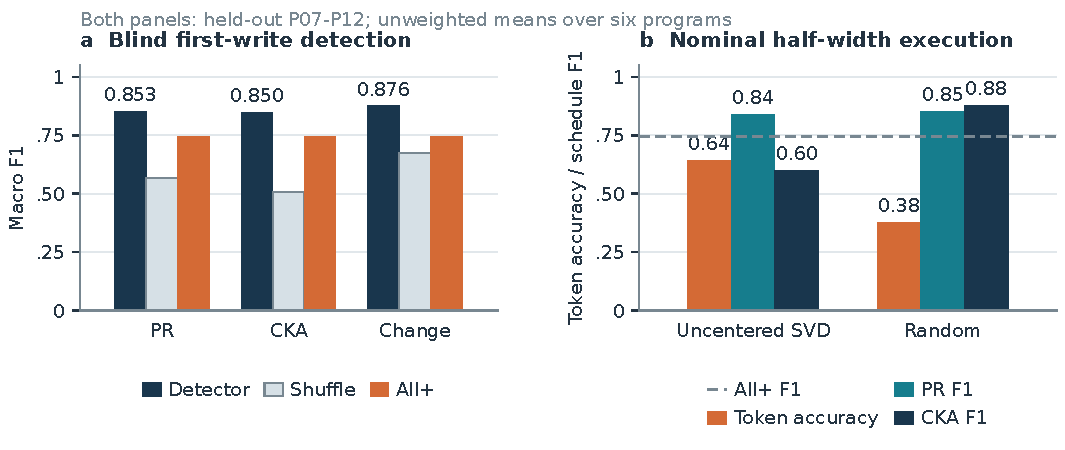
\includegraphics[width=.94\linewidth]{figures/fig1-recovery-compression.pdf}
\captionof{figure}{Both panels average the six held-out programs. Random half-width compression scores 0.879 CKA F1 against the original intended schedule while task accuracy is only 37.62\%. That schedule is not known causal ground truth for the changed model.}
\end{center}

\heading{Limits and conclusion}
The original fidelity benchmark still uses compiler-known lanes and write times. PR depends on encoding and scale. PCA-to-variable mapping is supervised; 60 undefined counterfactual condition rows remain failures. P11 CKA does not beat its always-write baseline. Erasure, lifetimes, and full circuit recovery are not established. InterpBench provides known circuits through SIIT; our ordinarily trained models do not inherit that ground truth. No direct InterpBench benchmark was run.

\heading{Evidence}
\begingroup\footnotesize\raggedright
Recorded verification includes 28 passing tests, five notebooks/37 cells, and 36 checkpoint replays. No scientific experiment was rerun for this brief.
\href{https://github.com/raghulchandramouli/RaspFormer/tree/e06479ce09f10695aa5280162f80d880c060eaf5}{RaspFormer code and canonical results, commit e06479c};
\href{https://arxiv.org/abs/2301.05062}{Tracr, Lindner et al., 2023};
\href{https://arxiv.org/abs/1905.00414}{CKA, Kornblith et al., 2019};
\href{https://doi.org/10.52202/079017-2950}{InterpBench, Gupta et al., 2024}.
\endgroup
\end{document}
